\documentclass[aspectratio=169,t]{beamer}
%\documentclass[aspectratio=43,t,handout]{beamer}

\usepackage[ansinew]{inputenc}
\usepackage[T1]{fontenc}
%English version FAU Logo
\usepackage[english]{babel}
%German version FAU Logo
%\usepackage[ngerman]{babel}
\usepackage{amsmath,amssymb}
\usepackage{graphicx}
\usepackage{listings}
\usepackage[backend=biber,sorting=none,doi=true,style=ieee]{biblatex}

\lstdefinelanguage
  [x64]{Assembler}     % add a "x64" dialect of Assembler
  [x86masm]{Assembler} % based on the "x86masm" dialect
  % with these extra keywords:
  {
    morekeywords={VMOVDQU,VPADDD,VPCMPEQB,VPXORD,VGATHERDPD,
                  CDQE,CQO,CMPSQ,CMPXCHG16B,JRCXZ,LODSQ,MOVSXD,
                  POPFQ,PUSHFQ,SCASQ,STOSQ,IRETQ,RDTSCP,SWAPGS,
                  rax,rdx,rcx,rbx,rsi,rdi,rsp,rbp,
                  r8,r8d,r8w,r8b,r9,r9d,r9w,r9b,
                  r10,r10d,r10w,r10b,r11,r11d,r11w,r11b,
                  r12,r12d,r12w,r12b,r13,r13d,r13w,r13b,
                  r14,r14d,r14w,r14b,r15,r15d,r15w,r15b,
                  k0,k1,k2,k3,k4,k5,k6,k7,k8,k9,k10,
                  xmm0,xmm1,xmm2,xmm3,xmm4,xmm5,xmm6,xmm7,xmm8,xmm9,xmm10,xmm11,xmm12,xmm13,xmm14,xmm15,xmm16,xmm17,xmm18,
                  ymm0,ymm1,ymm2,ymm3,ymm4,ymm5,ymm6,ymm7,ymm8,ymm9,ymm10,ymm11,ymm12,ymm13,ymm14,ymm15,ymm16,ymm17,ymm18,
                  zmm0,zmm1,zmm2,zmm3,zmm4,zmm5,zmm6,zmm7,zmm8,zmm9,zmm10,zmm11,zmm12,zmm13,zmm14,zmm15,zmm16,zmm17,zmm18},
    morecomment=[l]{\#}
  }

% Themes:
%  - fau:          FAU theme
%  - fau-med:      MedFak FAU theme
%  - fau-nat:      NatFak FAU theme
%  - fau-phil:     PhilFak FAU theme
%  - fau-rw:       RWFak FAU theme
%  - fau-rw-jura:  RWFak FB Jura FAU theme
%  - fau-rw-wiso:  RWFak FB WISO FAU theme
%  - fau-tf:       TechFak FAU theme
%
% Options:
%  - image:        Cover image on title page
%  - plain:        Plain title page
%  - longtitle:    Title page layout for long title
\usetheme[longtitle]{fau}

% Enable semi-transparent animation preview
\setbeamercovered{transparent}

\lstset{%
  language=C,
  tabsize=2,
  basicstyle=\tt\scriptsize,
  keywordstyle=\color{blue},
  commentstyle=\color{green!50!black},
  stringstyle=\color{red},
  keywords=[2]{computeForce},
  keywords=[3]{reneighbour},
  keywordstyle=[2]{\color{red!100!black}},
  keywordstyle=[3]{\color{green!50!black}},
  aboveskip=0.0em,
  %numbers=left,
  %numbersep=0.5em,
  %numberstyle=\tt\tiny
}

\defbibheading{bibliography}{}
\addbibresource[label=primary]{references.bib}
\nocite{*}


% Title, authors, and date
\title[MD Performance Analysis]{Current State of Performance Analysis for Molecular Dynamics}
\author[Rafael Ravedutti L. Machado, Jan Eitzinger]{Rafael Ravedutti L. Machado, Jan Eitzinger}
% English version
\institute[NHR@FAU]{Erlangen National High Performance Computing Center (NHR@FAU)}
% German version
%\institute[Lehrstuhl f\"ur XYZ]{Lehrstuhl f\"ur XYZ, Friedrich-Alexander-Universit\"at Erlangen-N\"urnberg}
\date{\today}
% Set additional logo (overwrites FAU seal)
%\logo{\includegraphics[width=.15\textwidth]{themefau/art/xxx/xxx.pdf}}


\begin{document}
  % Title
  \maketitle

  { % Motivation
    \setbeamertemplate{footline}{}
    \begin{frame}[noframenumbering]{Idea:}
        \begin{itemize}
            \item Separate contributions:
            \begin{itemize}
                \item Core execution
                \item Bandwidth
                \item Latency
            \end{itemize}
            \item Correlate core execution measurements with IACA and OSACA outputs
            \item "Randomness" of MD accesses
            \item Understand the generated assembly
            \item Explore and compare performance for different strategies
        \end{itemize}
    \end{frame}
  }
  \begin{frame}[noframenumbering]{Progress so far:}
      \begin{itemize}
          \item MD-Bench
          \begin{itemize}
              \item AoS and SoA layouts
              \item Different atom types
              \item Stubbed force calculation within cache sizes
          \end{itemize}
          \item Gather Benchmark
          \begin{itemize}
              \item Written in pure assembly
              \item AoS and SoA variants for MD
          \end{itemize}
          \item OSACA and IACA Analysis
          \item Analysis of Assembly
          \begin{itemize}
              \item Three variants
              \item "Prefetching" instructions
              \item Software vs Hardware Gathers
          \end{itemize}
      \end{itemize}
  \end{frame}

  % First, talk about MD-Bench, what it is, what it computes, how it works and etc
  % Talk about our changes: AoS Layout, multiple data types and stubbed force benchmark
  % we want to evaluate the cost of gathers
  % Show structure of the code
  % Show force calculation
  % Talk about the Assembly analysis of MD-Bench
  % Then, talk about the gather-bench, first gather version and md-variants with SoA and AoS
  % Which results to show?

  \begin{frame}[fragile]{MD-Bench}
    \begin{itemize}
      \item \url{https://github.com/RRZE-HPC/MD-Bench}
      \item Sequential re-implementation of miniMD in C
      \item Aim: as simple, clear and understandable as possible
      \item \textbf{Features:}
      \begin{itemize}
        \item Standard test case (Cu FCC lattice)
        \item Lennard Jones potential
        \item Full neighbor lists
      \end{itemize}
      \item \textbf{Runtime Parameters:}
      \begin{itemize}
        \item Number of timesteps
        \item Number of unit cells in x, y and y dimensions 
      \end{itemize}
      \item 4 atoms per unit cell with about 64 neighbors per atom
      \item Improvements:
      \begin{itemize}
        \item Stubbed force-calculation to run within L1, L2 and L3 caches
        \item Choose data layouts for atoms during compile-time (AoS vs SoA)
        \item Allow multiple atom types for simulation.
      \end{itemize}
    \end{itemize}
  \end{frame}

  \begin{frame}[fragile]{Simulation Loop}
    \begin{lstlisting}
for(int n = 0; n < param.ntimes; n++) {
  initialIntegrate(&param, &atom);
  if((n + 1) % param.every) {
    updatePbc(&atom, &param);
  } else {
    reneighbour(&param, &atom, &neighbor);
  }
  computeForce(&param, &atom, &neighbor);
  finalIntegrate(&param, &atom);
  if(!((n + 1) % param.nstat) && (n+1) < param.ntimes) {
    computeThermo(n + 1, &param, &atom);
  }
}
    \end{lstlisting}
    \begin{itemize}
      \item Computing the forces is normally the most expensive part!
      \item Building the neighbor lists can also take a considerable fraction of the simulation time, specially when:
      \begin{itemize}
        \item Force calculation time gets smaller (simpler potential to compute, optimizations)
        \item Rebuilding frequency gets smaller!
      \end{itemize}
      \item \textbf{For now, we just focus on the force computation!}
    \end{itemize}
  \end{frame}

  \begin{frame}[fragile]{Force Computation Loop}
    \vspace{-15.5pt}
    \begin{lstlisting}[basicstyle=\tt\tiny]
for(int i = 0; i < Nlocal; i++) { // 131072 for standard case
  neighs = &neighbor->neighbors[i * neighbor->maxneighs];
  int numneighs = neighbor->numneigh[i];
  MD_FLOAT xtmp = atom_x(i);
  MD_FLOAT ytmp = atom_y(i);
  MD_FLOAT ztmp = atom_z(i);
  MD_FLOAT fix = 0;
  MD_FLOAT fiy = 0;
  MD_FLOAT fiz = 0;

  for(int k = 0; k < numneighs; k++) { // average of 64 neighbors per atom
    int j = neighs[k];
    MD_FLOAT delx = xtmp - atom_x(j);
    MD_FLOAT dely = ytmp - atom_y(j);
    MD_FLOAT delz = ztmp - atom_z(j);
    MD_FLOAT rsq = delx * delx + dely * dely + delz * delz;
    if(rsq < cutforcesq) {
      MD_FLOAT sr2 = 1.0 / rsq;
      MD_FLOAT sr6 = sr2 * sr2 * sr2 * sigma6;
      MD_FLOAT force = 48.0 * sr6 * (sr6 - 0.5) * sr2 * epsilon;
      fix += delx * force;
      fiy += dely * force;
      fiz += delz * force;
    }
  }

  fx[i] += fix, fy[i] += fiy, fz[i] += fiz;
}
    \end{lstlisting}
  \end{frame}

  \begin{frame}[fragile]{Neighbors Loop}
    \begin{lstlisting}
for(int k = 0; k < numneighs; k++) {
  int j = neighs[k];
  MD_FLOAT delx = xtmp - atom_x(j);
  MD_FLOAT dely = ytmp - atom_y(j);
  MD_FLOAT delz = ztmp - atom_z(j);
  MD_FLOAT rsq = delx * delx + dely * dely + delz * delz;
  if(rsq < cutforcesq) {
    MD_FLOAT sr2 = 1.0 / rsq;
    MD_FLOAT sr6 = sr2 * sr2 * sr2 * sigma6;
    MD_FLOAT force = 48.0 * sr6 * (sr6 - 0.5) * sr2 * epsilon;
    fix += delx * force;
    fiy += dely * force;
    fiz += delz * force;
  }
}
    \end{lstlisting}
    \begin{itemize}
      \item To vectorize the code for \texttt{k}, gathering of the data is required
      \item Two possibilities: Hardware or Software gather
    \end{itemize}
  \end{frame}

  \begin{frame}[fragile]{Hardware vs. Software gather}
    \begin{itemize}
      \item \textbf{Hardware:} use asm \texttt{vgather} instructions
      \item \textbf{Software:} manually do gather operations with vloadunpack, permutations and swizzles
      \begin{itemize}
        \item Take advantage of data locality on AoS
        \item Probably better for out-of-order execution as well (several instructions vs. one gather)
      \end{itemize}
      \item For MD-Bench, all generated kernels (both AoS and SoA) for AVX512 use hardware gathers
    \end{itemize}
  \end{frame}

  \begin{frame}[fragile]{Hardware vs. Software gather}
  \centering
    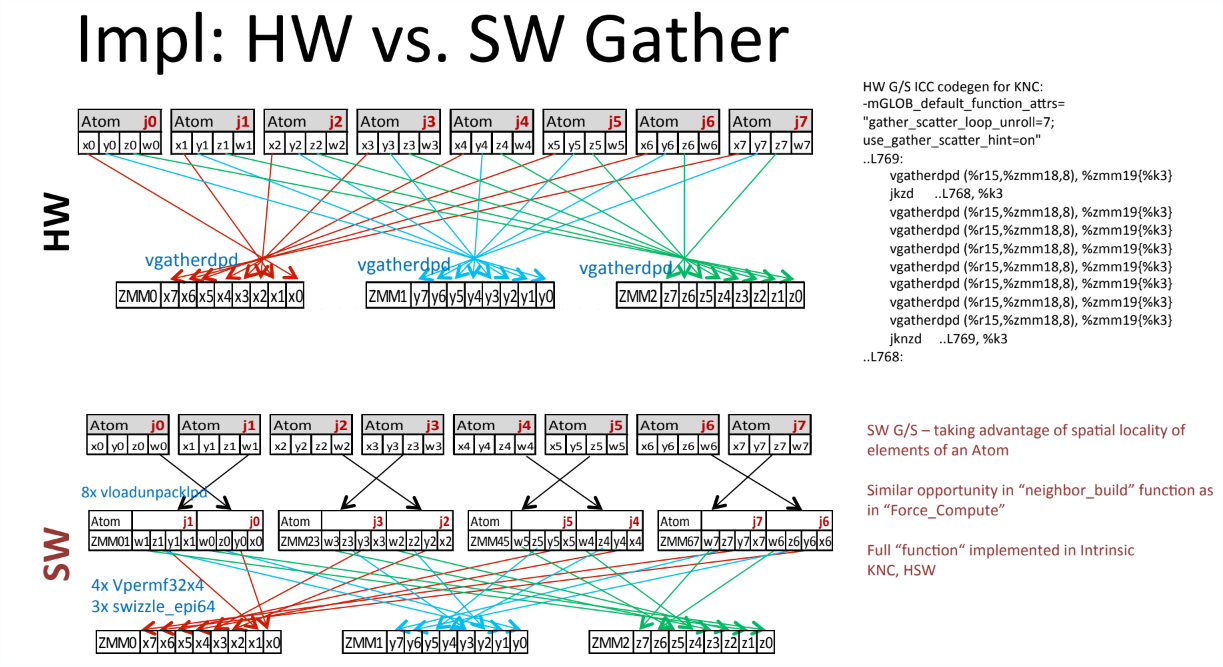
\includegraphics[width=12cm]{hw_vs_sw_gather_md.png}
  \end{frame}

  \begin{frame}[fragile]{Hardware vs. Software gather}
  \centering
    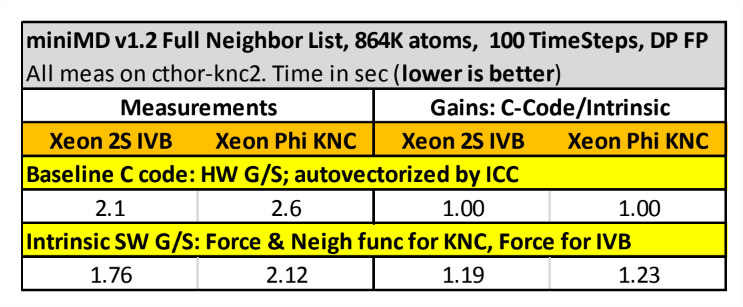
\includegraphics[width=10cm]{minimd_hw_vs_sw_results_table.png}
  \end{frame}

  \begin{frame}[fragile]{Assembly Analysis}
    \begin{itemize}
      \item Intel compiler (ICC) v19.0.5.281 Build 20190815
      \item Flags: \texttt{-S -masm=intel -D\_GNU\_SOURCE -DAOS -DPRECISION=2 -DALIGNMENT=64 -restrict -Ofast -xCORE-AVX 512 -qopt-zmm-usage=high -o ICC/force.s}
      \item For AVX512, all kernels with zmm registers and gather instructions
      \item Three kernel variants are generated by the compiler (Consider \texttt{rmng\_neighs = numneighs - k}):
      \begin{itemize}
        \item \texttt{rmng\_neighs < 8:} last iteration, vectors are not fulfilled
        \item \texttt{rmng\_neighs in ]8, 1200]:} with mov+lea instructions (prefetching?), L1 case? 1200 * 3 * 8 = 28.8kB, L1 cache size is 32kB on Cascade Lake
        \item \texttt{rmng\_neighs >= 1200:} no mov+lea instructions
      \end{itemize}
      \item We will focus on the \texttt{rmng\_neighs in ]8, 1200]} variant
    \end{itemize}
  \end{frame}

  \begin{frame}[fragile]{Assembly Analysis:}
    \vspace{-17.5pt}
    \begin{lstlisting}[language={[x64]Assembler},basicstyle=\tt\tiny]
vmovdqu   ymm3, YMMWORD PTR [r13+rbx*4]         # ymm3 <- neighs[k]
vpaddd    ymm4, ymm3, ymm3                      # ymm4 <- neighs[k] * 2
vpaddd    ymm3, ymm3, ymm4                      # ymm3 <- neighs[k] * 3
# -------------------- mov+lea instructions (prefetching?) -----------------------
mov       r10d, DWORD PTR [r13+rbx*4]           # r10d <- neighs[k]
mov       r9d, DWORD PTR [4+r13+rbx*4]          # r9d  <- neighs[k + 1]
mov       r8d, DWORD PTR [8+r13+rbx*4]          # r8d  <- neighs[k + 2]
mov       esi, DWORD PTR [12+r13+rbx*4]         # esi  <- neighs[k + 3]
lea       r10d, DWORD PTR [r10+r10*2]           # r10d <- neighs[k] * 3
mov       ecx, DWORD PTR [16+r13+rbx*4]         # ecx  <- neighs[k + 4]
lea       r9d, DWORD PTR [r9+r9*2]              # r9d  <- neighs[k + 1] * 3
mov       edx, DWORD PTR [20+r13+rbx*4]         # edx  <- neighs[k + 5]
lea       r8d, DWORD PTR [r8+r8*2]              # r8d  <- neighs[k + 2] * 3
mov       eax, DWORD PTR [24+r13+rbx*4]         # edx  <- neighs[k + 6]
lea       esi, DWORD PTR [rsi+rsi*2]            # esi  <- neighs[k + 3] * 3
mov       r15d, DWORD PTR [28+r13+rbx*4]        # edx  <- neighs[k + 7]
lea       ecx, DWORD PTR [rcx+rcx*2]            # ecx  <- neighs[k + 4] * 3
lea       edx, DWORD PTR [rdx+rdx*2]            # edx  <- neighs[k + 5] * 3
lea       eax, DWORD PTR [rax+rax*2]            # eax  <- neighs[k + 6] * 3
lea       r15d, DWORD PTR [r15+r15*2]           # r15d <- neighs[k + 7] * 3
# -------------------- end of mov+lea instructions -------------------------------
vpcmpeqb  k1, xmm0, xmm0                        # k1    <- [true for all elements]
vpcmpeqb  k2, xmm0, xmm0                        # k2    <- [true for all elements]
vpcmpeqb  k3, xmm0, xmm0                        # k3    <- [true for all elements]
vpxord    zmm4, zmm4, zmm4                      # zmm4  <- 0.0
vpxord    zmm17, zmm17, zmm17                   # zmm17 <- 0.0
vpxord    zmm18, zmm18, zmm18                   # zmm18 <- 0.0
vgatherdpd zmm4{k1}, QWORD PTR [16+rdi+ymm3*8]  # zmm4  <- atom->x[j * 3 + 2]
vgatherdpd zmm17{k2}, QWORD PTR [8+rdi+ymm3*8]  # zmm17 <- atom->x[j * 3 + 1]
vgatherdpd zmm18{k3}, QWORD PTR [rdi+ymm3*8]    # zmm18 <- atom->x[j * 3]
    \end{lstlisting}
  \end{frame}

  \begin{frame}[fragile]{Assembly Analysis:}
    When removing mov+lea instructions, performance is better on Cascade Lake:
    \begin{verbatim}
    With lea+mov:
    TOTAL 9.30s FORCE 4.81s NEIGH 4.25s REST 0.24s

    Without lea+mov:
    TOTAL 8.95s FORCE 4.43s NEIGH 4.28s REST 0.24s
    \end{verbatim}
  \end{frame}

  \begin{frame}[fragile]{Stubbed Force Calculation}
    \begin{itemize}
      \item Goal: core execution time contribution
      \item Execute most internal loop with data fitting into cache sizes
      \item Keep number of neighbors per atom fixed
      \item Compare cycles per iteration with OSACA and IACA outputs
    \end{itemize}
  \end{frame}

  \begin{frame}{Stubbed Force Calculation}
  \centering
    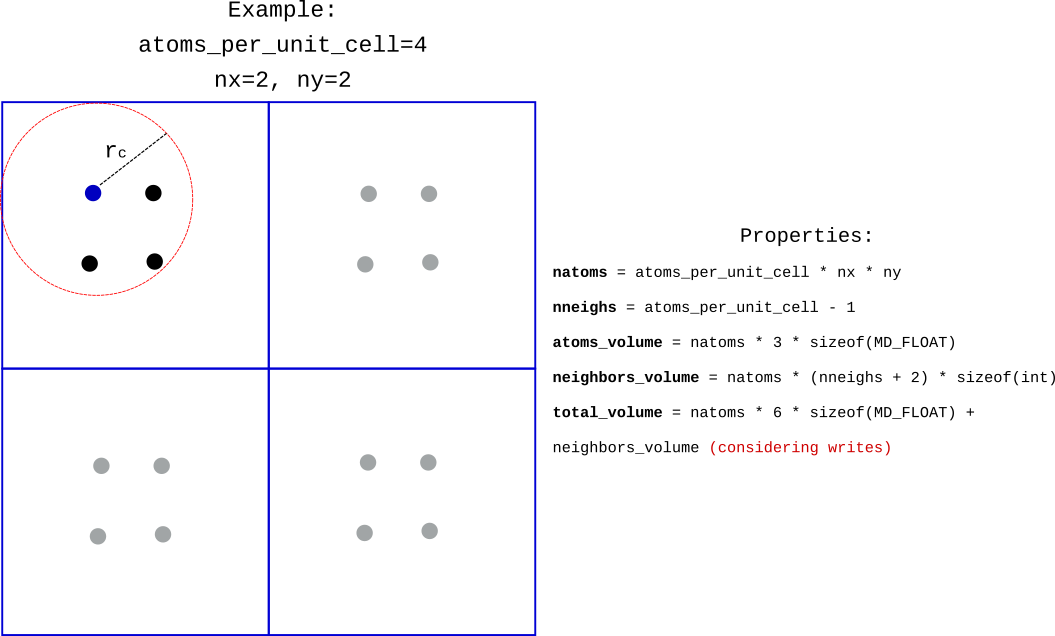
\includegraphics[width=11cm]{stubbed_force_mdbench.png}
  \end{frame}

  \begin{frame}[fragile]{OSACA Analysis}
    \vspace{-20pt}
    \begin{lstlisting}[basicstyle=\tt\fontsize{4pt}{6pt}\selectfont]
                                     Port pressure in cycles
 0   - 0DV  |  1   |  2   -  2D  |  3   -  3D  |  4   |  5   |  6   |  7   ||  CP  | LCD  |
-------------------------------------------------------------------------------------------------
            |      |             |             |      |      |      |      ||      |      | X vpcmpeqb  %xmm0, %xmm0, %k2
0.00        | 0.50 |             |             |      | 0.00 | 0.50 |      ||      |      |   addl      $8, %r9d
            |      |             |             |      |      |      |      ||      |      | X vpcmpeqb  %xmm0, %xmm0, %k1
            |      |             |             |      |      |      |      ||      |      | X vpcmpeqb  %xmm0, %xmm0, %k3
            |      | 0.50   0.50 | 0.50   0.50 |      |      |      |      ||  4.0 |      |   vmovdqu   (%rcx,%r14,4), %ymm3
0.00        | 0.50 |             |             |      | 0.00 | 0.50 |      ||      |      |   addq      $8, %r14
0.50        |      |             |             |      | 0.50 |      |      ||      |      |   vpxord    %zmm5, %zmm5, %zmm5
0.50        |      |             |             |      | 0.50 |      |      ||      |      |   vpxord    %zmm4, %zmm4, %zmm4
0.50        |      |             |             |      | 0.50 |      |      ||      |      |   vpxord    %zmm6, %zmm6, %zmm6
1.50        | 0.50 | 4.00   0.50 | 4.00   0.50 |      | 0.50 | 0.50 |      ||  4.0 |      |   vgatherdpd (%rax,%ymm3,8), %zmm5{%k2}
1.50        | 0.50 | 4.00   0.50 | 4.00   0.50 |      | 0.50 | 0.50 |      ||      |      |   vgatherdpd (%rdx,%ymm3,8), %zmm4{%k1}
1.50        | 0.50 | 4.00   0.50 | 4.00   0.50 |      | 0.50 | 0.50 |      ||      |      |   vgatherdpd (%rsi,%ymm3,8), %zmm6{%k3}
0.50        |      |             |             |      | 0.50 |      |      ||  4.0 |      |   vsubpd    %zmm5, %zmm1, %zmm29
0.50        |      |             |             |      | 0.50 |      |      ||      |      |   vsubpd    %zmm4, %zmm0, %zmm28
0.50        |      |             |             |      | 0.50 |      |      ||      |      |   vsubpd    %zmm6, %zmm2, %zmm31
0.50        |      |             |             |      | 0.50 |      |      ||  4.0 |      |   vmulpd    %zmm29, %zmm29, %zmm20
0.50        |      |             |             |      | 0.50 |      |      ||  4.0 |      |   vfmadd231pd %zmm28, %zmm28, %zmm20
0.50        |      |             |             |      | 0.50 |      |      ||  4.0 |      |   vfmadd231pd %zmm31, %zmm31, %zmm20
2.50        |      |             |             |      | 0.50 |      |      ||  8.0 |      |   vrcp14pd  %zmm20, %zmm27
            |      |             |             |      | 1.00 |      |      ||      |      |   vcmppd    $1, %zmm16, %zmm20, %k5
            |      |             |             |      | 1.00 |      |      ||      |      |   vfpclasspd $30, %zmm27, %k0
0.50        |      | 0.50   0.50 | 0.50   0.50 |      | 0.50 |      |      ||  4.0 |      |   vfnmadd213pd .L_2il0floatpacket.5(%rip){1to8}, %zmm27, %zmm20
1.00        |      |             |             |      |      |      |      ||      |      |   knotw     %k0, %k4
0.50        |      |             |             |      | 0.50 |      |      ||  4.0 |      |   vmulpd    %zmm20, %zmm20, %zmm21
0.50        |      |             |             |      | 0.50 |      |      ||      |      |   vfmadd213pd %zmm27, %zmm20, %zmm27{%k4}
0.50        |      |             |             |      | 0.50 |      |      ||  4.0 |      |   vfmadd213pd %zmm27, %zmm21, %zmm27{%k4}
0.50        |      |             |             |      | 0.50 |      |      ||  4.0 |      |   vmulpd    %zmm15, %zmm27, %zmm22
0.50        |      |             |             |      | 0.50 |      |      ||      |      |   vmulpd    %zmm14, %zmm27, %zmm24
0.50        |      |             |             |      | 0.50 |      |      ||  4.0 |      |   vmulpd    %zmm22, %zmm27, %zmm25
0.50        |      |             |             |      | 0.50 |      |      ||  4.0 |      |   vmulpd    %zmm25, %zmm27, %zmm23
0.50        |      |             |             |      | 0.50 |      |      ||      |      |   vfmsub213pd %zmm7, %zmm25, %zmm27
0.50        |      |             |             |      | 0.50 |      |      ||  4.0 |      |   vmulpd    %zmm24, %zmm23, %zmm26
0.00        |      |             |             |      | 1.00 |      |      ||  4.0 |      |   vmulpd    %zmm27, %zmm26, %zmm30
    \end{lstlisting}
  \end{frame}

  \begin{frame}[fragile]{OSACA Analysis}
    \vspace{-20pt}
    \begin{lstlisting}[basicstyle=\tt\fontsize{4pt}{6pt}\selectfont]
                                     Port pressure in cycles
 0   - 0DV  |  1   |  2   -  2D  |  3   -  3D  |  4   |  5   |  6   |  7   ||  CP  | LCD  |
-------------------------------------------------------------------------------------------------
0.00        |      |             |             |      | 1.00 |      |      ||      |      |   vfmadd231pd %zmm28, %zmm30, %zmm13{%k5}
0.00        |      |             |             |      | 1.00 |      |      ||      |  4.0 |   vfmadd231pd %zmm29, %zmm30, %zmm12{%k5}
0.00        |      |             |             |      | 1.00 |      |      ||  4.0 |      |   vfmadd231pd %zmm31, %zmm30, %zmm11{%k5}
0.00        | 0.50 |             |             |      | 0.00 | 0.50 |      ||      |      |   cmpl      %ebx, %r9d
            |      |             |             |      |      |      |      ||      |      | * jb        ..B1.22       # Prob 82%

17.5          3.00   13.0   2.50   13.0   2.50          17.5   3.00           68.0    4


Loop-Carried Dependencies Analysis Report
-----------------------------------------
 1.0 | addl      $8, %r9d                                      | [257]
 1.0 | addq      $8, %r14                                      | [261]
 4.0 | vfmadd231pd %zmm29, %zmm30, %zmm12{%k5}                 | [290]
 4.0 | vfmadd231pd %zmm28, %zmm30, %zmm13{%k5}                 | [289]
 4.0 | vfmadd231pd %zmm31, %zmm30, %zmm11{%k5}                 | [291]
    \end{lstlisting}
  \end{frame}

  \begin{frame}[fragile]{IACA Analysis}
    \vspace{-20pt}
    \begin{lstlisting}[basicstyle=\tt\fontsize{4pt}{6pt}\selectfont]
Throughput Analysis Report
--------------------------
Block Throughput: 36.70 Cycles       Throughput Bottleneck: Backend
Loop Count:  23
Port Binding In Cycles Per Iteration:
--------------------------------------------------------------------------------------------------
|  Port  |   0   -  DV   |   1   |   2   -  D    |   3   -  D    |   4   |   5   |   6   |   7   |
--------------------------------------------------------------------------------------------------
| Cycles | 17.5     0.0  | 11.0  | 20.5    17.0  | 20.5    17.0  |  7.0  | 20.5  |  7.0  |  0.0  |
--------------------------------------------------------------------------------------------------
...
| Num Of   |                    Ports pressure in cycles                         |      |
|  Uops    |  0  - DV    |  1   |  2  -  D    |  3  -  D    |  4   |  5   |  6   |  7   |
-----------------------------------------------------------------------------------------
|   1*     |             |      |             |             |      |      |      |      | mov r13, r8
|   1      |             | 1.0  |             |             |      |      |      |      | imul r13, rcx
|   1      |             |      |             |             |      | 1.0  |      |      | vbroadcastsd zmm2, xmm6
|   1      |             |      |             |             |      | 1.0  |      |      | vbroadcastsd zmm1, xmm7
|   1      |             |      |             |             |      | 1.0  |      |      | vbroadcastsd zmm0, xmm12
|   1      |             |      |             |             |      |      | 1.0  |      | movsxd rbx, r12d
|   1      |             |      |             |             |      |      | 1.0  |      | add r13, r10
|   2^     |             |      | 0.5         | 0.5         | 1.0  |      |      |      | mov qword ptr [rsp-0x40], rax
|   2^     |             |      | 0.5         | 0.5         | 1.0  |      |      |      | mov qword ptr [rsp-0x38], r8
|   2^     |             |      | 0.5         | 0.5         | 1.0  |      |      |      | mov qword ptr [rsp-0x30], r10
|   2^     |             |      | 0.5         | 0.5         | 1.0  |      |      |      | mov qword ptr [rsp-0x28], rsi
|   2^     |             |      | 0.5         | 0.5         | 1.0  |      |      |      | mov qword ptr [rsp-0x20], rcx
|   2^     |             |      | 0.5         | 0.5         | 1.0  |      |      |      | mov qword ptr [rsp-0x50], r9
|   2^     |             |      | 0.5         | 0.5         | 1.0  |      |      |      | mov qword ptr [rsp-0x48], rdx
|   1      |             |      | 0.5     0.5 | 0.5     0.5 |      |      |      |      | vmovdqu ymm3, ymmword ptr [r13+rbx*4]
|   1      |             | 1.0  |             |             |      |      |      |      | vpaddd ymm4, ymm3, ymm3
|   1      |             | 1.0  |             |             |      |      |      |      | vpaddd ymm3, ymm3, ymm4
|   1      |             |      | 0.5     0.5 | 0.5     0.5 |      |      |      |      | mov r10d, dword ptr [r13+rbx*4]
|   1      |             |      | 0.5     0.5 | 0.5     0.5 |      |      |      |      | mov r9d, dword ptr [r13+rbx*4+0x4]
|   1      |             |      | 0.5     0.5 | 0.5     0.5 |      |      |      |      | mov r8d, dword ptr [r13+rbx*4+0x8]
|   1      |             |      | 0.5     0.5 | 0.5     0.5 |      |      |      |      | mov esi, dword ptr [r13+rbx*4+0xc]
|   1      |             | 1.0  |             |             |      |      |      |      | lea r10d, ptr [r10+r10*2]
|   1      |             |      | 0.5     0.5 | 0.5     0.5 |      |      |      |      | mov ecx, dword ptr [r13+rbx*4+0x10]
|   1      |             | 1.0  |             |             |      |      |      |      | lea r9d, ptr [r9+r9*2]
    \end{lstlisting}
  \end{frame}

  \begin{frame}[fragile]{IACA Analysis}
    \vspace{-20pt}
    \begin{lstlisting}[basicstyle=\tt\fontsize{4pt}{6pt}\selectfont]
|   1      |             |      | 0.5     0.5 | 0.5     0.5 |      |      |      |      | mov edx, dword ptr [r13+rbx*4+0x14]
|   1      |             | 1.0  |             |             |      |      |      |      | lea r8d, ptr [r8+r8*2]
|   1      |             |      | 0.5     0.5 | 0.5     0.5 |      |      |      |      | mov eax, dword ptr [r13+rbx*4+0x18]
|   1      |             | 1.0  |             |             |      |      |      |      | lea esi, ptr [rsi+rsi*2]
|   1      |             |      | 0.5     0.5 | 0.5     0.5 |      |      |      |      | mov r15d, dword ptr [r13+rbx*4+0x1c]
|   1      |             | 1.0  |             |             |      |      |      |      | lea ecx, ptr [rcx+rcx*2]
|   1      |             | 1.0  |             |             |      |      |      |      | lea edx, ptr [rdx+rdx*2]
|   1      |             | 1.0  |             |             |      |      |      |      | lea eax, ptr [rax+rax*2]
|   1      |             | 1.0  |             |             |      |      |      |      | lea r15d, ptr [r15+r15*2]
|   1      |             |      |             |             |      | 1.0  |      |      | vpcmpeqb k1, xmm0, xmm0
|   1      |             |      |             |             |      | 1.0  |      |      | vpcmpeqb k2, xmm0, xmm0
|   1      |             |      |             |             |      | 1.0  |      |      | vpcmpeqb k3, xmm0, xmm0
|   1*     |             |      |             |             |      |      |      |      | vpxord zmm4, zmm4, zmm4
|   1*     |             |      |             |             |      |      |      |      | vpxord zmm17, zmm17, zmm17
|   1*     |             |      |             |             |      |      |      |      | vpxord zmm18, zmm18, zmm18
|   5^     | 2.0         |      | 4.0     4.0 | 4.0     4.0 |      |      | 1.0  |      | vgatherdpd zmm4, k1, zmmword ptr [rdi+ymm3*8+0x10]
|   5^     | 1.5         |      | 4.0     4.0 | 4.0     4.0 |      | 0.5  | 1.0  |      | vgatherdpd zmm17, k2, zmmword ptr [rdi+ymm3*8+0x8]
|   5^     | 1.0         |      | 4.0     4.0 | 4.0     4.0 |      | 1.0  | 1.0  |      | vgatherdpd zmm18, k3, zmmword ptr [rdi+ymm3*8]
|   1      |             |      |             |             |      |      | 1.0  |      | add r12d, 0x8
|   1      |             |      |             |             |      |      | 1.0  |      | add rbx, 0x8
|   1      | 0.5         |      |             |             |      | 0.5  |      |      | vsubpd zmm26, zmm0, zmm4
|   1      | 0.5         |      |             |             |      | 0.5  |      |      | vsubpd zmm24, zmm1, zmm17
|   1      | 0.5         |      |             |             |      | 0.5  |      |      | vsubpd zmm23, zmm2, zmm18
|   1      | 0.5         |      |             |             |      | 0.5  |      |      | vmulpd zmm3, zmm24, zmm24
|   1      | 0.5         |      |             |             |      | 0.5  |      |      | vfmadd231pd zmm3, zmm23, zmm23
|   1      | 0.5         |      |             |             |      | 0.5  |      |      | vfmadd231pd zmm3, zmm26, zmm26
|   3      | 2.0         |      |             |             |      | 1.0  |      |      | vrcp14pd zmm22, zmm3
|   1      |             |      |             |             |      | 1.0  |      |      | vcmppd k2, zmm3, zmm14, 0x1
|   1      |             |      |             |             |      | 1.0  |      |      | vfpclasspd k0, zmm22, 0x1e
|   2^     | 1.0         |      | 0.5     0.5 | 0.5     0.5 |      |      |      |      | vfnmadd213pd zmm3, zmm22, qword ptr [rip]{1to8}
|   1      | 1.0         |      |             |             |      |      |      |      | knotw k1, k0
|   1      |             |      |             |             |      | 1.0  |      |      | vmulpd zmm4, zmm3, zmm3
|   1      | 0.5         |      |             |             |      | 0.5  |      |      | vfmadd213pd zmm22{k1}, zmm3, zmm22
|   1      | 0.5         |      |             |             |      | 0.5  |      |      | vfmadd213pd zmm22{k1}, zmm4, zmm22
|   1      | 0.5         |      |             |             |      | 0.5  |      |      | vmulpd zmm17, zmm22, zmm13
|   1      | 0.5         |      |             |             |      | 0.5  |      |      | vmulpd zmm19, zmm22, zmm10
|   1      | 0.5         |      |             |             |      | 0.5  |      |      | vmulpd zmm20, zmm22, zmm17
|   1      | 0.5         |      |             |             |      | 0.5  |      |      | vmulpd zmm18, zmm22, zmm20
    \end{lstlisting}
  \end{frame}

  \begin{frame}[fragile]{IACA Analysis}
    \vspace{-20pt}
    \begin{lstlisting}[basicstyle=\tt\fontsize{4pt}{6pt}\selectfont]
|   1      | 0.5         |      |             |             |      | 0.5  |      |      | vfmsub213pd zmm22, zmm20, zmm5
|   1      | 0.5         |      |             |             |      | 0.5  |      |      | vmulpd zmm21, zmm18, zmm19
|   1      | 0.5         |      |             |             |      | 0.5  |      |      | vmulpd zmm25, zmm21, zmm22
|   1      | 0.5         |      |             |             |      | 0.5  |      |      | vfmadd231pd zmm9{k2}, zmm25, zmm23
|   1      | 0.5         |      |             |             |      | 0.5  |      |      | vfmadd231pd zmm8{k2}, zmm25, zmm24
|   1      | 0.5         |      |             |             |      | 0.5  |      |      | vfmadd231pd zmm11{k2}, zmm25, zmm26
|   1*     |             |      |             |             |      |      |      |      | cmp r12d, r14d
|   0*F    |             |      |             |             |      |      |      |      | jb 0xfffffffffffffed3
Total Num Of Uops: 91
Analysis Notes:
Backend allocation was stalled due to unavailable allocation resources.
There were bubbles in the frontend.
    \end{lstlisting}
  \end{frame}

  \begin{frame}[fragile]{Cycles per iteration with AoS AVX512 kernels}
    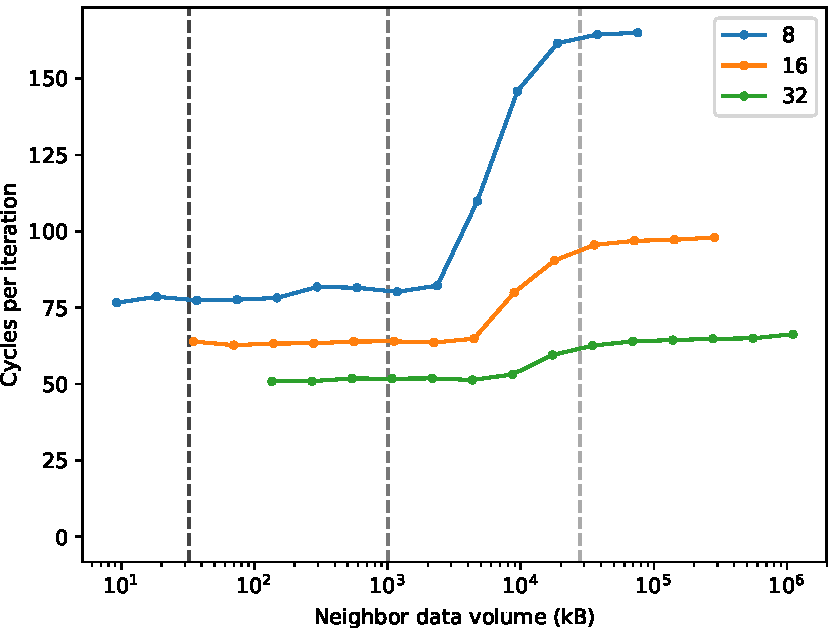
\includegraphics[width=9cm]{results_aos_casclakesp2_neighbor_vol.pdf}
  \end{frame}

  \begin{frame}[fragile]{Cycles per iteration with SoA AVX512 kernels}
    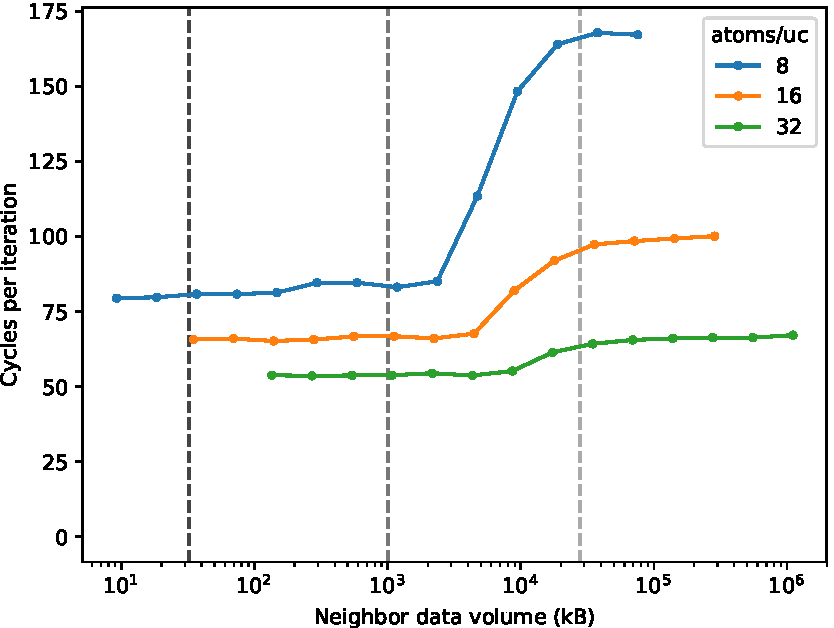
\includegraphics[width=9cm]{results_soa_casclakesp2_neighbor_vol.pdf}
  \end{frame}

  \begin{frame}[fragile]{}
    \begin{itemize}
      \item \textbf{Issue: internal loop is not executed enough times for each atom!}
      \item Overhead to fill pipeline with instructions has a considerable effect on the cycles per iteration!
      \item Cycles measured for some cases are considerably higher than OSACA/IACA predictions!
      \item \textbf{Solution: repeat the most internal loop}
    \end{itemize}
  \end{frame}

  \begin{frame}[fragile]{Neighbors Loop}
    \begin{lstlisting}
...
for(int n = 0; n < ntimes; n++) {
  for(int k = 0; k < numneighs; k++) {
    int j = neighs[k];
    MD_FLOAT delx = xtmp - atom_x(j);
    MD_FLOAT dely = ytmp - atom_y(j);
    MD_FLOAT delz = ztmp - atom_z(j);
    MD_FLOAT rsq = delx * delx + dely * dely + delz * delz;

    if(rsq < cutforcesq) {
      MD_FLOAT sr2 = 1.0 / rsq;
      MD_FLOAT sr6 = sr2 * sr2 * sr2 * sigma6;
      MD_FLOAT force = 48.0 * sr6 * (sr6 - 0.5) * sr2 * epsilon;
      fix += delx * force;
      fiy += dely * force;
      fiz += delz * force;
    }
  }
}
...
    \end{lstlisting}
  \end{frame}

  \begin{frame}[fragile]{Cycles per iteration with SoA AVX512 kernels (repeating internal loop)}
    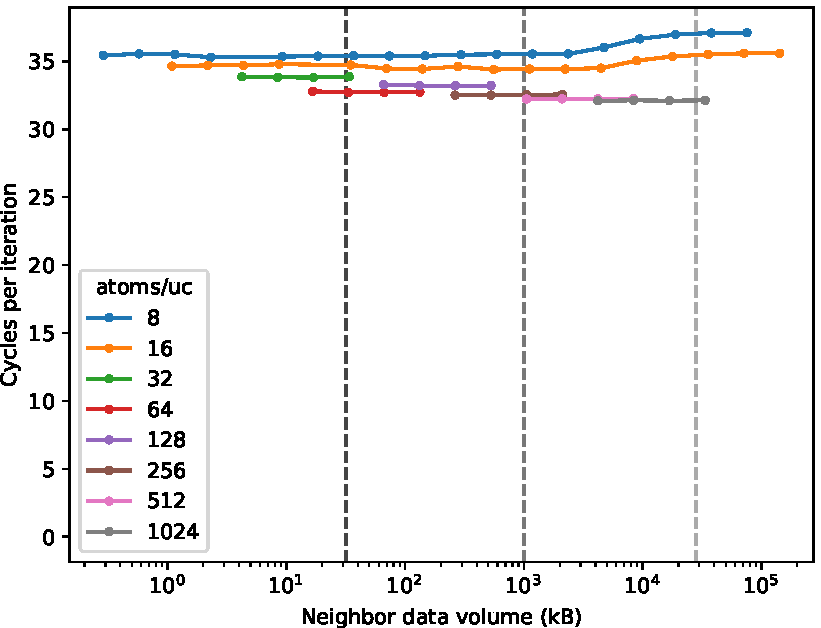
\includegraphics[width=9cm]{results_soa_casclakesp2_rep_neighbor_vol.pdf}
  \end{frame}

  \begin{frame}[fragile]{Stubbed Force Calculation}
    \begin{itemize}
      \item Require internal loop repetition to provide more accurate results
      \item Increasing the atoms per unit cells (\# neighbors) reduces cycles per iteration
      \begin{itemize}
        \item Until which point?
      \end{itemize}
      \item \textbf{Is there a better way to measure core execution contribution?}
      \item What about data traffic contributions?
    \end{itemize}
  \end{frame}

  \begin{frame}[fragile]{gather-bench}
    \begin{itemize}
      \item Benchmark for gathering data into registers
      \item Measure impact of gathers with several data volumes with respect to cache lines touched
      \item Input: stride of elements to be gathered
      \item Support for AVX2 and AVX512 (currently)
      \item Based on previous benchmark, some changes:
      \begin{itemize}
        \item Gather kernels explicitly written in Assembly
        \item MD variants: AoS and SoA
        \item Tests for correctness
      \end{itemize}
      \item Next steps to implement: SW gathers, evaluate with lea+mov instructions
    \end{itemize}
  \end{frame}

  \begin{frame}[fragile]{AVX512 Gather (simple array):}
    \vspace{-17.5pt}
    \begin{lstlisting}[language={[x64]Assembler},basicstyle=\tt\tiny]
...
xor   rax, rax
.align 16
1:
vpcmpeqb k1, xmm0, xmm0
vpcmpeqb k2, xmm0, xmm0
vpcmpeqb k3, xmm0, xmm0
vpcmpeqb k4, xmm0, xmm0
vmovdqu ymm0, [rsi + rax*4]
vmovdqu ymm1, [rsi + rax*4+32]
vmovdqu ymm2, [rsi + rax*4+64]
vmovdqu ymm3, [rsi + rax*4+96]
vpxord zmm4, zmm4, zmm4
vpxord zmm5, zmm5, zmm5
vpxord zmm6, zmm6, zmm6
vpxord zmm7, zmm7, zmm7
vgatherdpd zmm4{k1}, [rdi + ymm0*8]
vgatherdpd zmm5{k2}, [rdi + ymm1*8]
vgatherdpd zmm6{k3}, [rdi + ymm2*8]
vgatherdpd zmm7{k4}, [rdi + ymm3*8]

# Required for test
#vmovapd [rcx + rax*8],     zmm4
#vmovapd [rcx + rax*8+64],  zmm5
#vmovapd [rcx + rax*8+128], zmm6
#vmovapd [rcx + rax*8+192], zmm7

addq rax, 32
cmpq rax, rdx
jl 1b
...
    \end{lstlisting}
  \end{frame}

  \begin{frame}[fragile]{Results for simple array}
    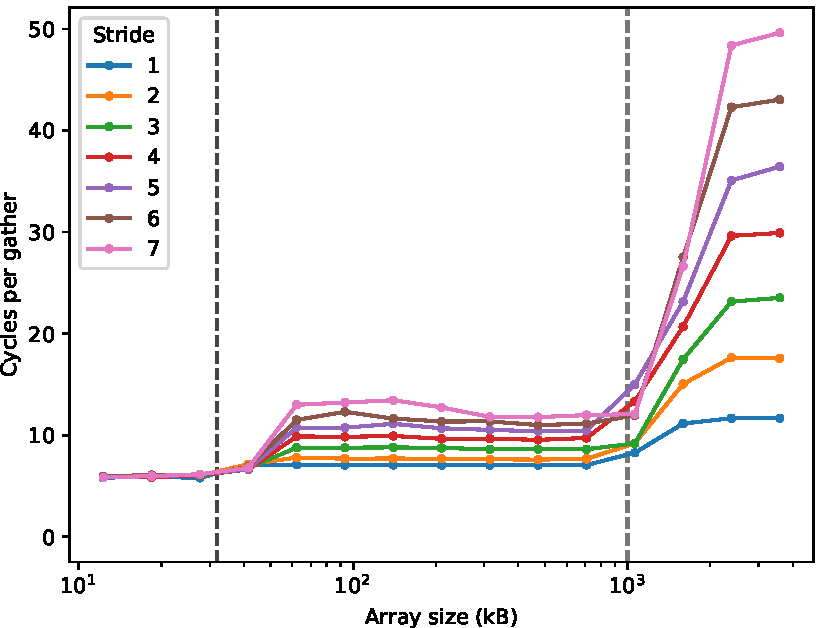
\includegraphics[width=9cm]{gather_casclakesp2_results.pdf}
  \end{frame}

  \begin{frame}[fragile]{AVX512 Gather (AoS):}
    \vspace{-17.5pt}
    \begin{lstlisting}[language={[x64]Assembler},basicstyle=\tt\tiny]
...
xor   rax, rax
.align 16
1:

vmovdqu ymm3, YMMWORD PTR [rsi + rax * 4]
vpaddd ymm4, ymm3, ymm3
vpaddd ymm3, ymm3, ymm4
vpcmpeqb k1, xmm5, xmm5
vpcmpeqb k2, xmm5, xmm5
vpcmpeqb k3, xmm5, xmm5
vpxord zmm0, zmm0, zmm0
vpxord zmm1, zmm1, zmm1
vpxord zmm2, zmm2, zmm2
vgatherdpd zmm0{k1}, [rdi + ymm3*8]
vgatherdpd zmm1{k2}, [8 + rdi + ymm3*8]
vgatherdpd zmm2{k3}, [16 + rdi + ymm3*8]

# Required for test
#vmovupd [rcx + rax*8], zmm0
#lea rbx, [rcx + rdx*8]
#vmovupd [rbx + rax*8], zmm1
#lea r9, [rbx + rdx*8]
#vmovupd [r9 + rax*8], zmm2

addq rax, 8
cmpq rax, rdx
jl 1b
...
    \end{lstlisting}
  \end{frame}

  \begin{frame}[fragile]{Results for AoS}
    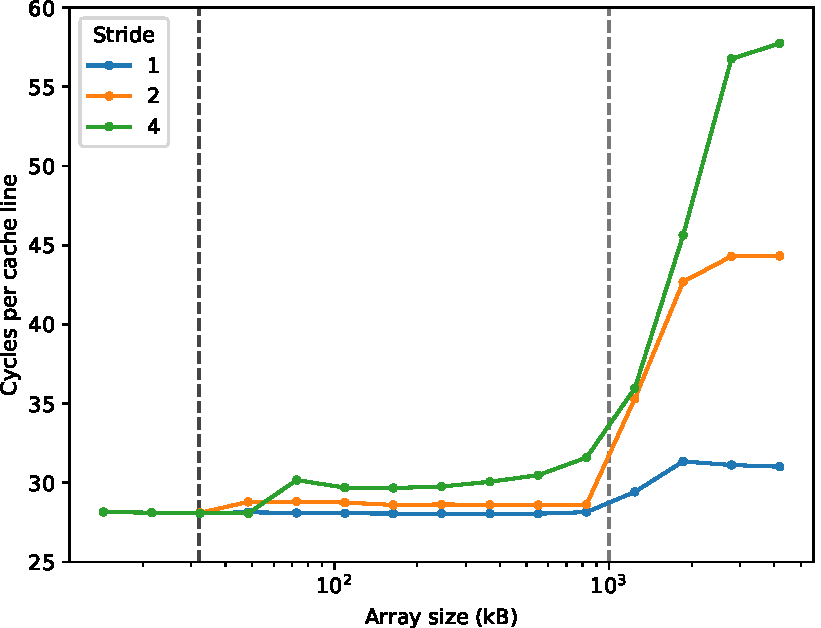
\includegraphics[width=9cm]{gather_md_skylakesp2_results.pdf}
  \end{frame}

  \begin{frame}[fragile]{Conclusion}
    \begin{itemize}
      \item Measure contributions:
      \begin{itemize}
        \item Core execution (stubbed force)
        \item Latency and Bandwidth (gather-bench)
      \end{itemize}
      \item Correlate "randomness" of memory access in MD to memory contributions
      \begin{itemize}
        \item Irregular accesses on gather
        \item Cache simulator
        \item Reuse distance
      \end{itemize}
      \item Investigate performance for different strategies/choices:
      \begin{itemize}
        \item AoS vs SoA
        \item Compiler
        \item HW vs. SW gather
        \item Different potentials (EAM)
      \end{itemize}
    \end{itemize}
  \end{frame}

  % List example
  %\begin{frame}[fragile]{Capturing expressions}
  %  \begin{itemize}
  %      \item Operator overloading
  %      \item Vector operations are easily expressed
  %  \end{itemize}
  %\end{frame}

  % Code example
  %\begin{frame}[fragile]{Capturing expressions}
  %  \begin{lstlisting}
  %  \end{lstlisting}
  %\end{frame}

  % Image example
  %\begin{frame}{Experimental Results}
  %  \begin{block}{Weak Scaling Perfomance}
  %    \includegraphics[width=9cm]{results/weak_scaling.png}
  %  \end{block}
  %\end{frame}

  { % Questions?
    %\setbeamertemplate{footline}{}
    %\begin{frame}[c,noframenumbering]
    %  \begin{center}
    %    Thank you for listening.\\
    %    {\bf Any questions?}
    %  \end{center}
    %\end{frame}

    % References
    %\section*{References}
    %\begin{frame}[allowframebreaks,noframenumbering]{References}
    %  \printbibliography
    %\end{frame}
  }
\end{document}

